
\subsection{One Example}\label{subsec:SIRModel}
\label{subsec:shillerpound}
Here, we provide a specific example of an economic question formulated in a thoroughgoing epidemiological way.  Our present purpose is not to extract economic insights -- we do that in section~{\ref{subsec:assetprice}} below -- but simply to illustrate how the epidemiological toolkit works.

\href{https://github.com/iworld1991/EpiExp/blob/master/Literature/shiller1989survey.pdf}{\cite{shiller1989survey}} use an SIR model to capture how interest in particular stocks spreads;\ifInBook{\footnote{This paper builds on the earlier work comparing the efficient market hypothesis of stock prices and an alternative model incorporating social dynamics \href{https://github.com/iworld1991/EpiExp/blob/master/Literature/shiller1984stock.pdf}{\cite{shiller1984stock}}. }}
{\footnote{Our treatment makes two inconsequential modifications.  First, in order to be able to instantiate the model using the \href{https://ndlib.readthedocs.io/en/latest/}{\texttt{NDLib}} computational toolkit described below, we rewrite the originally continuous-time model in a discrete-time form. Second, the original paper described an additional stochastic shock to the change in $I_t$ meant to capture a potential ``change in the `source' of the infection or the nature of the contagion.''  Because that shock was not actually used for any results in the paper, we neglect it in our exposition.}}% CDC to TW: Make sure this is explained in the notebook. % We have had them in the notebook now.
 we examine a model almost identical to theirs.
At date  $t$, a large population of investors measured by the real number $N$ is divided into three ``compartments.''  (See Figure \ref{fig:sir_diagram}).  $I_t$ investors are currently ``infected'' with interest in a certain stock;  $S_t$ investors are not infected but are ``susceptible'' to becoming interested; and $R_t$ measures investors who have been ``infected'' but have ``recovered'' from the infection.\footnote{For our purposes here, we do not need to define the exact consequences of `recovery.'  See below (or see the original paper) for further discussion.}

Under `random mixing,' each person is expected to have contact with $\contactNum$ others, randomly selected from the entire population.  The only kind of contact with any consequence is between an infected and a susceptible person: Such an encounter has a probability $\tranProb$ of causing the susceptible person to become infected.

Epidemiological models typically define a parameter $\beta$ that combines consequences of the rate of social contact $\contactNum$ and the rate of transmission upon  contact, $\tranProb$:\ifInBook{}{\footnote{In any SIR model embedding an explicitly defined connection network by which the ``disease'' spreads, $\beta$ is the product of the average number of connected nodes (``degree''), and the infection probability conditional on contact. For instance, in a random graph (\cite{erdos1960evolution})  with connection probability $p$ and the size of network N, the average contacts every agent has is $(N-1)p$. }}
\begin{verbatimwrite}{./Equations/beta}
\begin{equation}
	\label{eq:beta}
    \beta  = \tranProb \contactNum.
\end{equation}
\end{verbatimwrite}
\begin{equation}
	\label{eq:beta}
    \beta  = \tranProb \contactNum.
\end{equation}


The expected number of new infections generated in period $t$ (corresponding to the decline in the number of susceptible persons) can now be calculated: Fraction $S_{t}/N$ of an infected person's contacts will be susceptible, so the number of newly generated infections per infected person will be $\tranProb \times \contactNum \times (S_{t}/N).$ The `infected' population also changes because every infected person recovers with a probability of $\gamma$ per period.

Putting these elements together, the  changes in the population in different compartments are given by
\begin{equation}
	\label{eq:sirdyn}
	\begin{split}
	&	\Delta S_{t+1} = -\beta I_{t}(S_{t}/N) \\
	&	\Delta I_{t+1} = \beta \frac{S_{t}}{N}I_{t} - \gamma I_t \\
&		\Delta \Recovered_{t+1} = \gamma I_t.
	\end{split}
\end{equation}

%The term $\beta \frac{S_{t}}{N}I_{t}$ captures the number of people who ``flow'' from ``compartment $S$'' to ``compartment $I$'', which is proportional to the infection rate $\beta$, the fraction of people who are susceptible $\frac{S_t}{N}$, and the number of the infected $I_t$. The  term $\gamma I_t$ captures the number of people who ``flow'' from $I$ to $\Recovered$


\begin{verbatimwrite}{./Slides/FigureSIRSimulation}%%%Slides
    \begin{figure} \centering  % [h!]  [!ht]
        \caption{ ~Simulated dynamics from a SIR model of stock investors}
        \label{fig:sir_simulate}
        \centerline{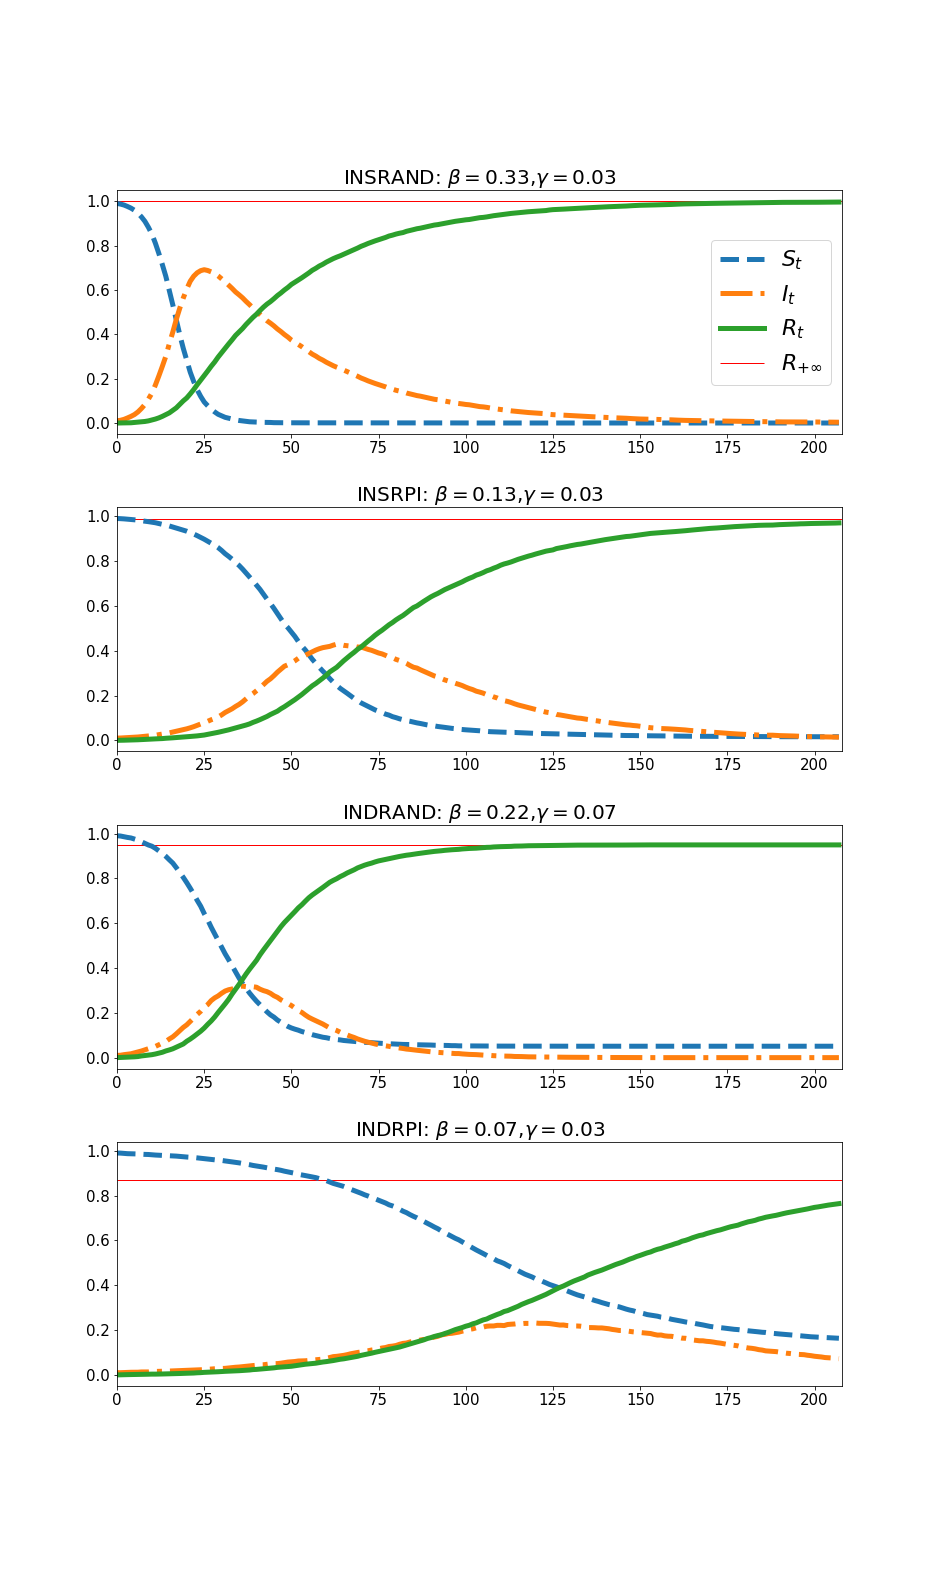
\includegraphics[width=0.85\textwidth,height=0.85\textheight]{./figures/sir_simulate}}
        \begin{flushleft}
            {\footnotesize The four figures respectively simulate an SIR model under calibrations corresponding to \cite{shiller1989survey}'s parameter estimates for (1) institutional investors for a randomly selected stock (INSRAND); (2) institutional investors for a rapidly rising stock (INSRPI); (3) individual investors for a random stock (INDRAND); and (4) individual investors for a rapidly rising stock (INDRPI). The susceptible population {\Susceptible} is dashed; dash-dot shows the size of the {\Infected} compartment, and the recovered population {\Recovered} is solid.  The horizontal thin solid line corresponds to the limiting size of compartment of $R$ in the long run.  To reproduce these figures, see the companion \href{https://github.com/llorracc/EpiExp/blob/master/SIR_Ndlib.ipynb}{Jupyter Notebook}. }
        \end{flushleft}
    \end{figure}
\end{verbatimwrite}%%%Slides
%%%Slides
  \begin{figure} \centering  % [h!]  [!ht]
    \caption{ ~Simulated dynamics from an SIR model of stock investors}
    \label{fig:sir_simulate}
    \centerline{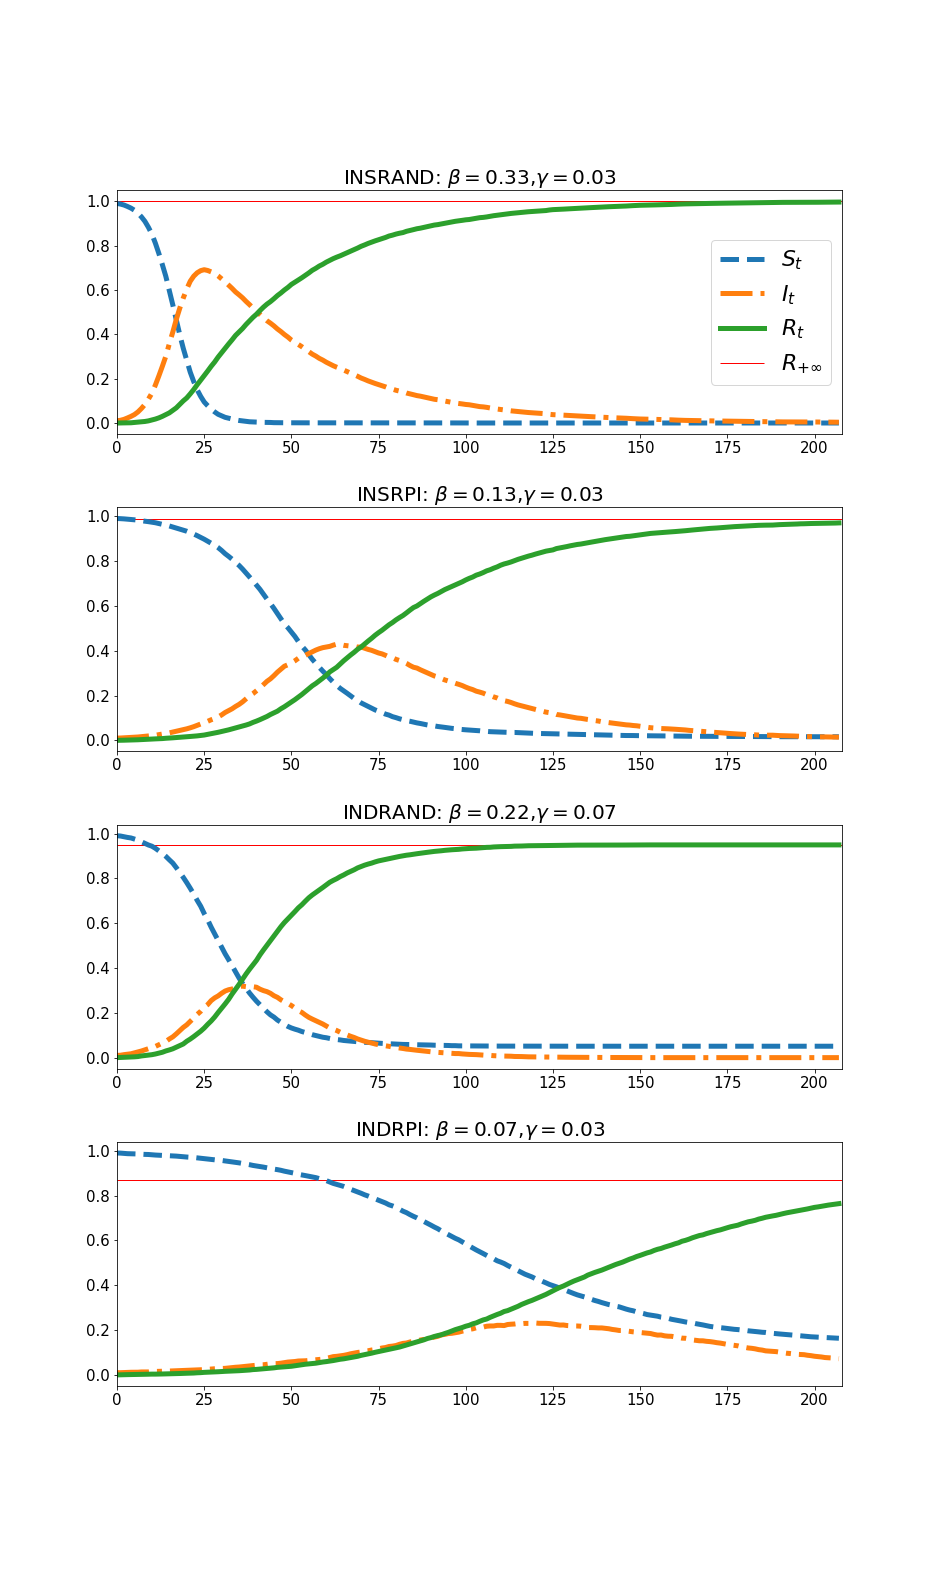
\includegraphics[width=0.85\textwidth,height=0.85\textheight]{./figures/sir_simulate}}
    \begin{flushleft}
      {\footnotesize Note: This graph plots the simulated paths of populations in different compartments in a SIR model of stock investors, as described in \cite{shiller1989survey}. We use the median estimates of the infection rate $\beta$ and recovery rate $\gamma$ for four samples: institutional investors for a randomly selected stock (INSRAND), institutional investors for a rapidly rising stock (INSRPI), individual investors for a random stock (INDRAND), and individual investors for a rapidly rising stock (INDRPI). The horizontal thin solid line corresponds to the limiting size of compartment of $R$ in the long run. The simulation is done with the Python library \href{https://ndlib.readthedocs.io/en/latest/}{``NDlib''}, for details, see the companion \href{https://github.com/llorracc/EpiExp/blob/master/SIR_Ndlib.ipynb}{Jupyter Notebook}. }
    \end{flushleft}
  \end{figure}
%%%Slides

The simplest special case of the SIR model is one with a recovery rate of $\gamma=0$, in which case the model reduces to the transmissible SI model discussed in Section \ref{subsec:epi_framework}.  Another straightforward case is $\beta < \gamma$, in which from any starting point the population of infected persons $I$ gradually dies down to zero.

\newcommand{\Rzero}{\mathcal{R}(0)}
The interesting cases emerge when the `basic reproduction ratio' $\Rzero = (\beta/\gamma)$ exceeds one (this $\Rzero$ is unrelated to the $\Recovered$ used elsewhere to measure the recovered population), because $\Rzero > 1$ guarantees that an initial arbitrarily small infection will grow, at least for a while (assuming that at the beginning everyone is susceptible, $S_{0}/N = 1$).

To illustrate the model's implications, we configure it with four combinations of parameter values taken from \cite{shiller1989survey}, characterizing two different kinds of investors and two categories of stocks.  %(Section~\ref{subsec:assetprice} describes the investors and stock categories, and interprets the economics; here we confine our observations to the epidemiology.)

\begin{verbatimwrite}{./Slides/FigureSIRFlowDiagram}%%%Slides
    \begin{figure}[!ht] \centering  % [h!]
        \caption{ ~A SIR model of stock investors}
        \label{fig:sir_diagram}
        \centerline{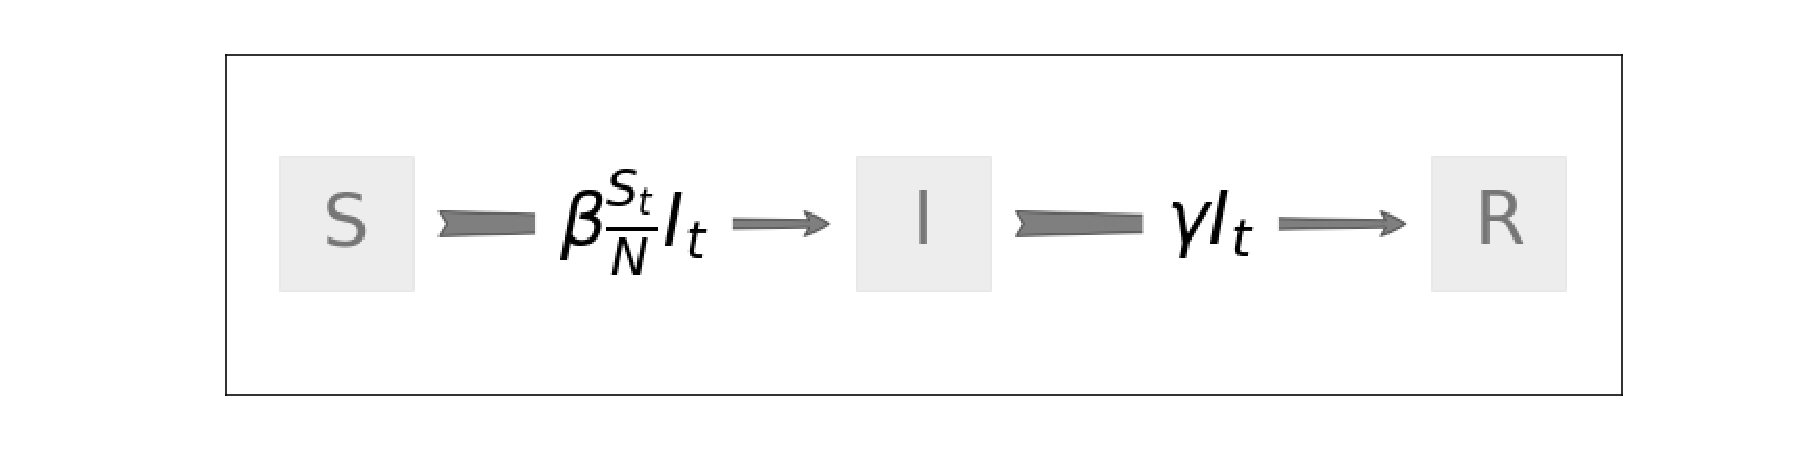
\includegraphics[width=\textwidth]{./figures/flow_diagram}}
        \begin{flushleft}
            {\footnotesize Note: This graph plots the transitions between different compartments in the SIR model of stock investors described in \cite{shiller1989survey}. }
        \end{flushleft}
    \end{figure}
\end{verbatimwrite}%%%Slides
%%%Slides
	\begin{figure}[!ht] \centering  % [h!]
		\caption{ ~A SIR model of stock investors}
		\label{fig:sir_diagram}
		\centerline{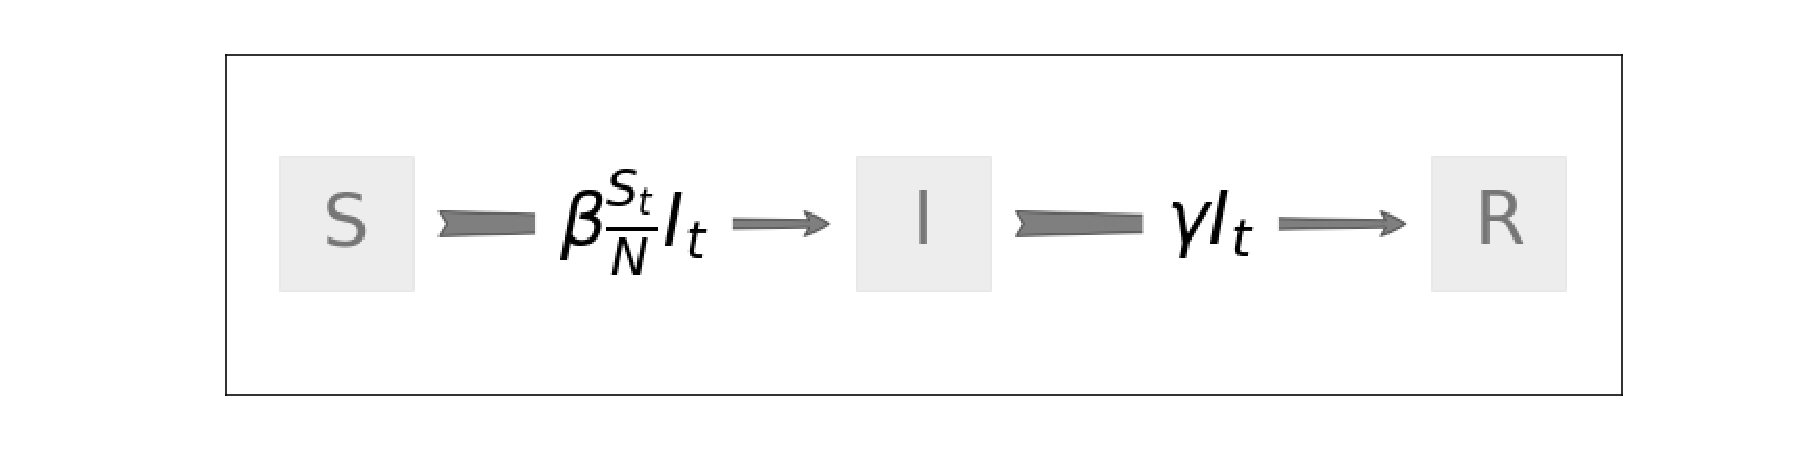
\includegraphics[width=1.5\textwidth]{./figures/flow_diagram}}
		\begin{flushleft}
			{\footnotesize Note: This graph plots the transitions between different compartments in the SIR model of stock investors described in \cite{shiller1989survey}. }
		\end{flushleft}
	\end{figure}


We calculate the quantitative implications using one of the best of the many computational toolkits for analyzing such models that have proliferated in recent years:  %\footnote{For the simulation of the SIR model we use the Python library \href{https://ndlib.readthedocs.io/en/latest/}{NDlib} (\cite{rossetti2018ndlib}), which builds upon another Python library called NetworkX (\cite{hagberg2008exploring}).}
\href{https://ndlib.readthedocs.io/en/latest/}{NDlib} lets users specify an arbitrary network structure on which a disease might spread. We exploit the above-mentioned fact that a random-mixing SIR model can be approximated with an \textit{ex-ante} generated random graph when the transmission probability $\tau$ and the average number of connections $\chi$ in the graph are configured such that their product is equal to the calibrated infection rate $\beta$ (see Equation \ref{eq:beta}).\footnote{See the companion \href{https://github.com/llorracc/EpiExp/blob/master/SIR_Ndlib.ipynb}{Jupyter Notebook} of this paper for our  implementation.}

In Figure \ref{fig:sir_simulate} the vertical axis measures the populations of {\Susceptible}, {\Infected}, and {\Recovered} investors; time since the initial date of infection is on the horizontal axis.  Also plotted is the limiting size of the recovered compartment\ifInBook{.}{, for which an analytical solution exists.\footnote{Given a constant basic reproduction ratio $\beta/\gamma$ that is strictly greater than $1$, and an initial fraction $S_{0}/N$ close to 1, the limiting fraction of $\Recovered$, denoted as $\recovered_{+\infty} = \Recovered_{+\infty}/N$, is the solution to the implicit equation: $e^{-\frac{\beta}{\gamma} r_{+\infty}} = 1-r_{+\infty}$.  See  \href{https://en.wikipedia.org/wiki/Compartmental_models_in_epidemiology\#Transition_rates}{this Wikipedia page}, \cite{harko2014exact}, \href{{https://iopscience.iop.org/article/10.1088/1751-8121/abc65d}}{\cite{kroger2020analytical}}, and \cite{okabe2021microscopic} for details of the results.}} % CDC to TW: Move the contents of this footnote to the Jupyter notebook (adding the papers to the nocite list)

Two common patterns emerge.  First, since in all four cases the basic reproduction ratio $\Rzero$ is greater than 1, in all four cases there is an outbreak. The size of the infected population first expands to its maximum value and then gradually levels off to zero, exhibiting a hump-shaped ``viral curve'' characteristic of SIR models.  Second, in all scenarios, the system ultimately converges to a steady-state where most people have cycled through infection and recovery. Even in the case with the smallest reproduction ratio, the proportion who cycle through the process of Infection and Recovery is almost 85 percent, implying a high degree of infectiousness. Under other configurations, the limiting size of the infected-then-recovered `compartment' $R$ is close to 100 percent.

The main difference in the parameterizations is the speed with which these eventualities play themselves out, which varies considerably.  (For a discussion of the model's economic (as distinct from epidemiological) content see Section~\ref{subsec:assetprice}).

%Even using the results of their own surveys explicitly designed for the purpose, \cite{shiller1989survey} needed to exercise considerable ingenuity to produce the calibrations we have used above.

%We highlight~\cite{shiller1989survey} here because it presents an early but rich example that satisfies all our criteria for an epidemiological model of economic expectations. First, it articulates and a explicit structural mathematical mechanism by which an idea (in this case, interest in a stock) spreads in the population as a result of social communication. Second, the model has clear assumptions and predictions for both the micro and macro dynamics of expectations, which can be tested (or calibrated) with measurable survey data (indeed, they were calibrated with data that~\cite{shiller1989survey} collected themselves because existing sources had not asked the right questions).  Third (as we explain in section~{\ref{subsec:assetprice}}), dynamics of separately measurable economic phenomena (stock prices) are hypothesized to be a consequence of the dynamics of those expectations.  % Not many papers satisfy all these criteria.

